\section{Particle ID}
\label{sec:Def_timing}

In this study, the benefit of the timing will be applied on tagging the particles. In the figures~\ref{Particle_ID_1}~\ref{Particle_ID_2}, they show the different kinds of the particles ID from trailing to next-to-next-to-next-to-next-to tailing ones. By comparing between two categories, T and PT trailing series, the extra 10\% protons could be tagged with the help of the timing.

\begin{figure}
\begin{center}
   \subfigure[Trailing-T] {
   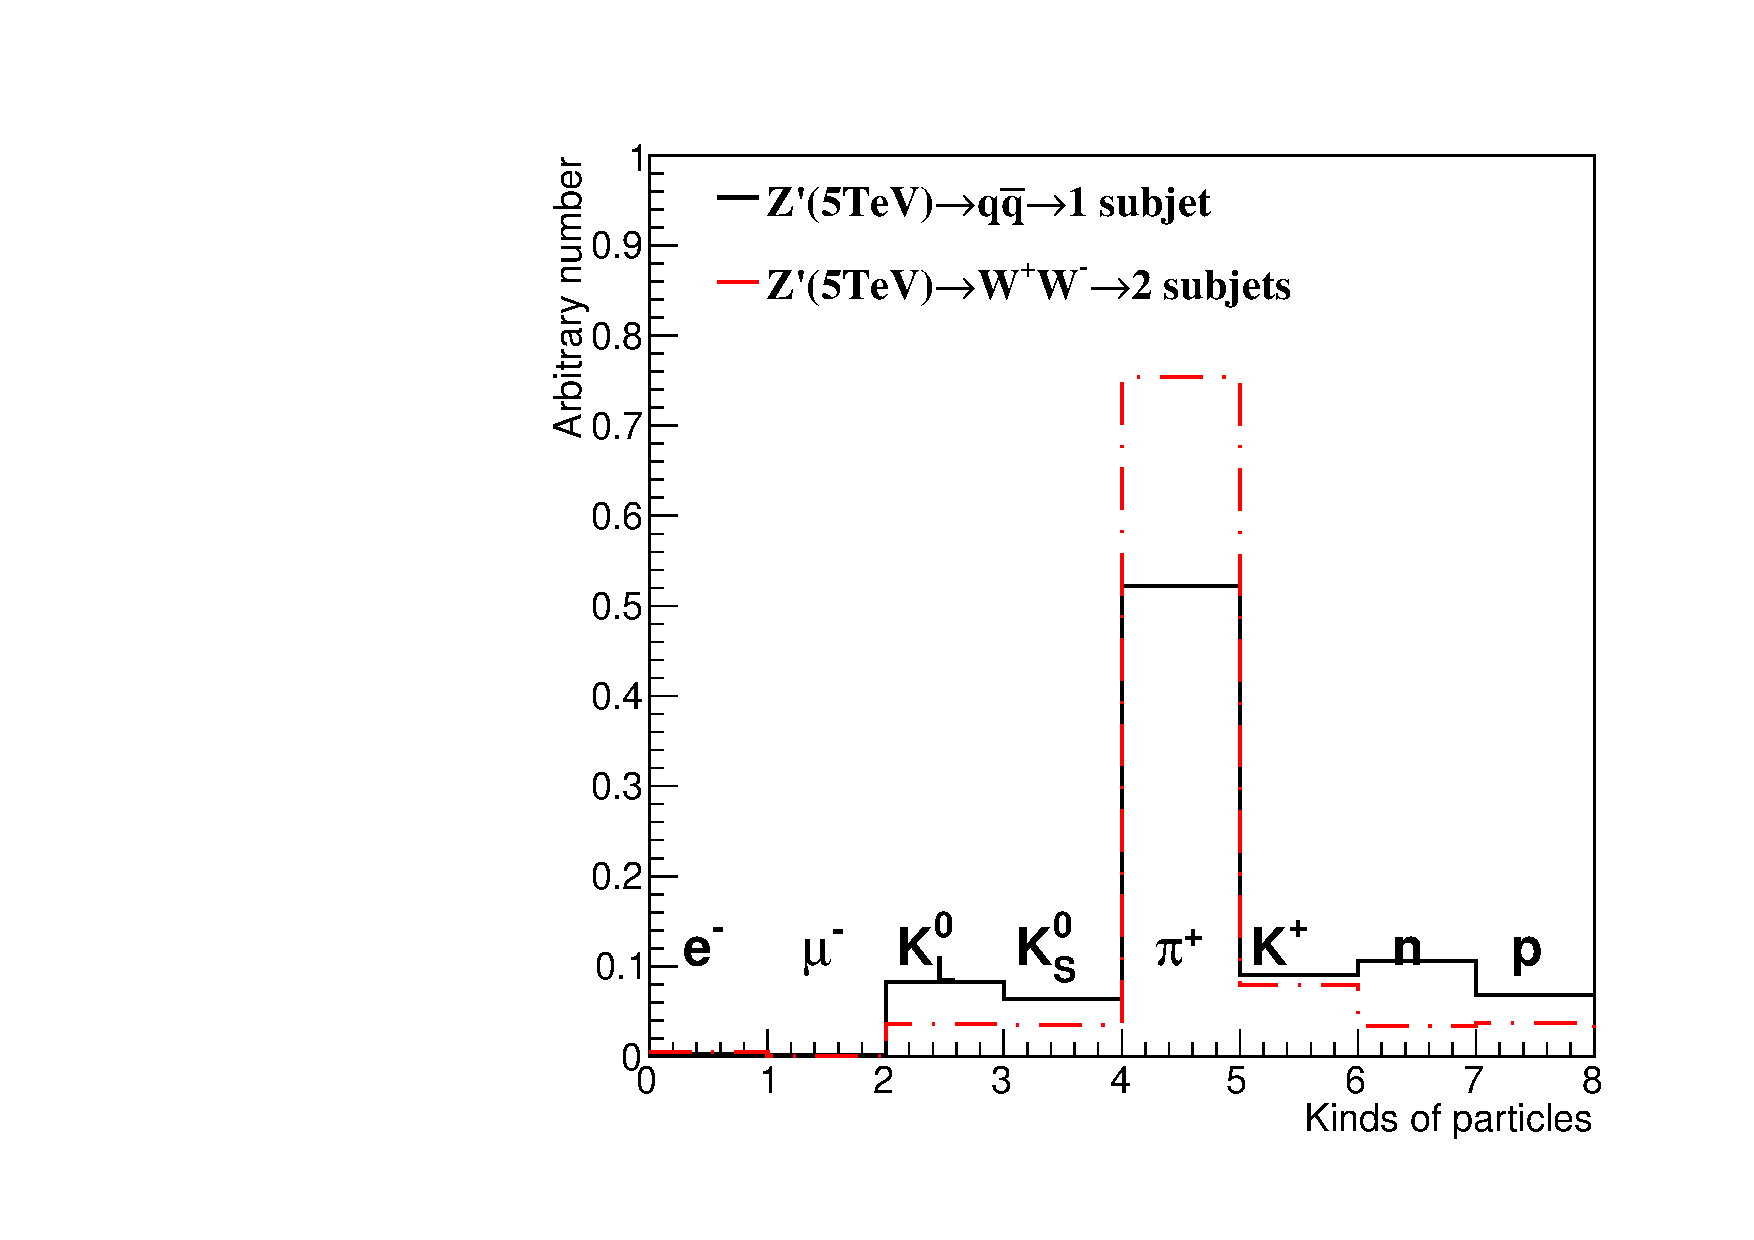
\includegraphics[width=0.45\textwidth]{/Users/ms08962476/singularity/TIming_Studies/Codes/5TeV/h_5TeV_Particles_Rank_T_0.pdf}
   }
   \subfigure[Trailing-PT] {
   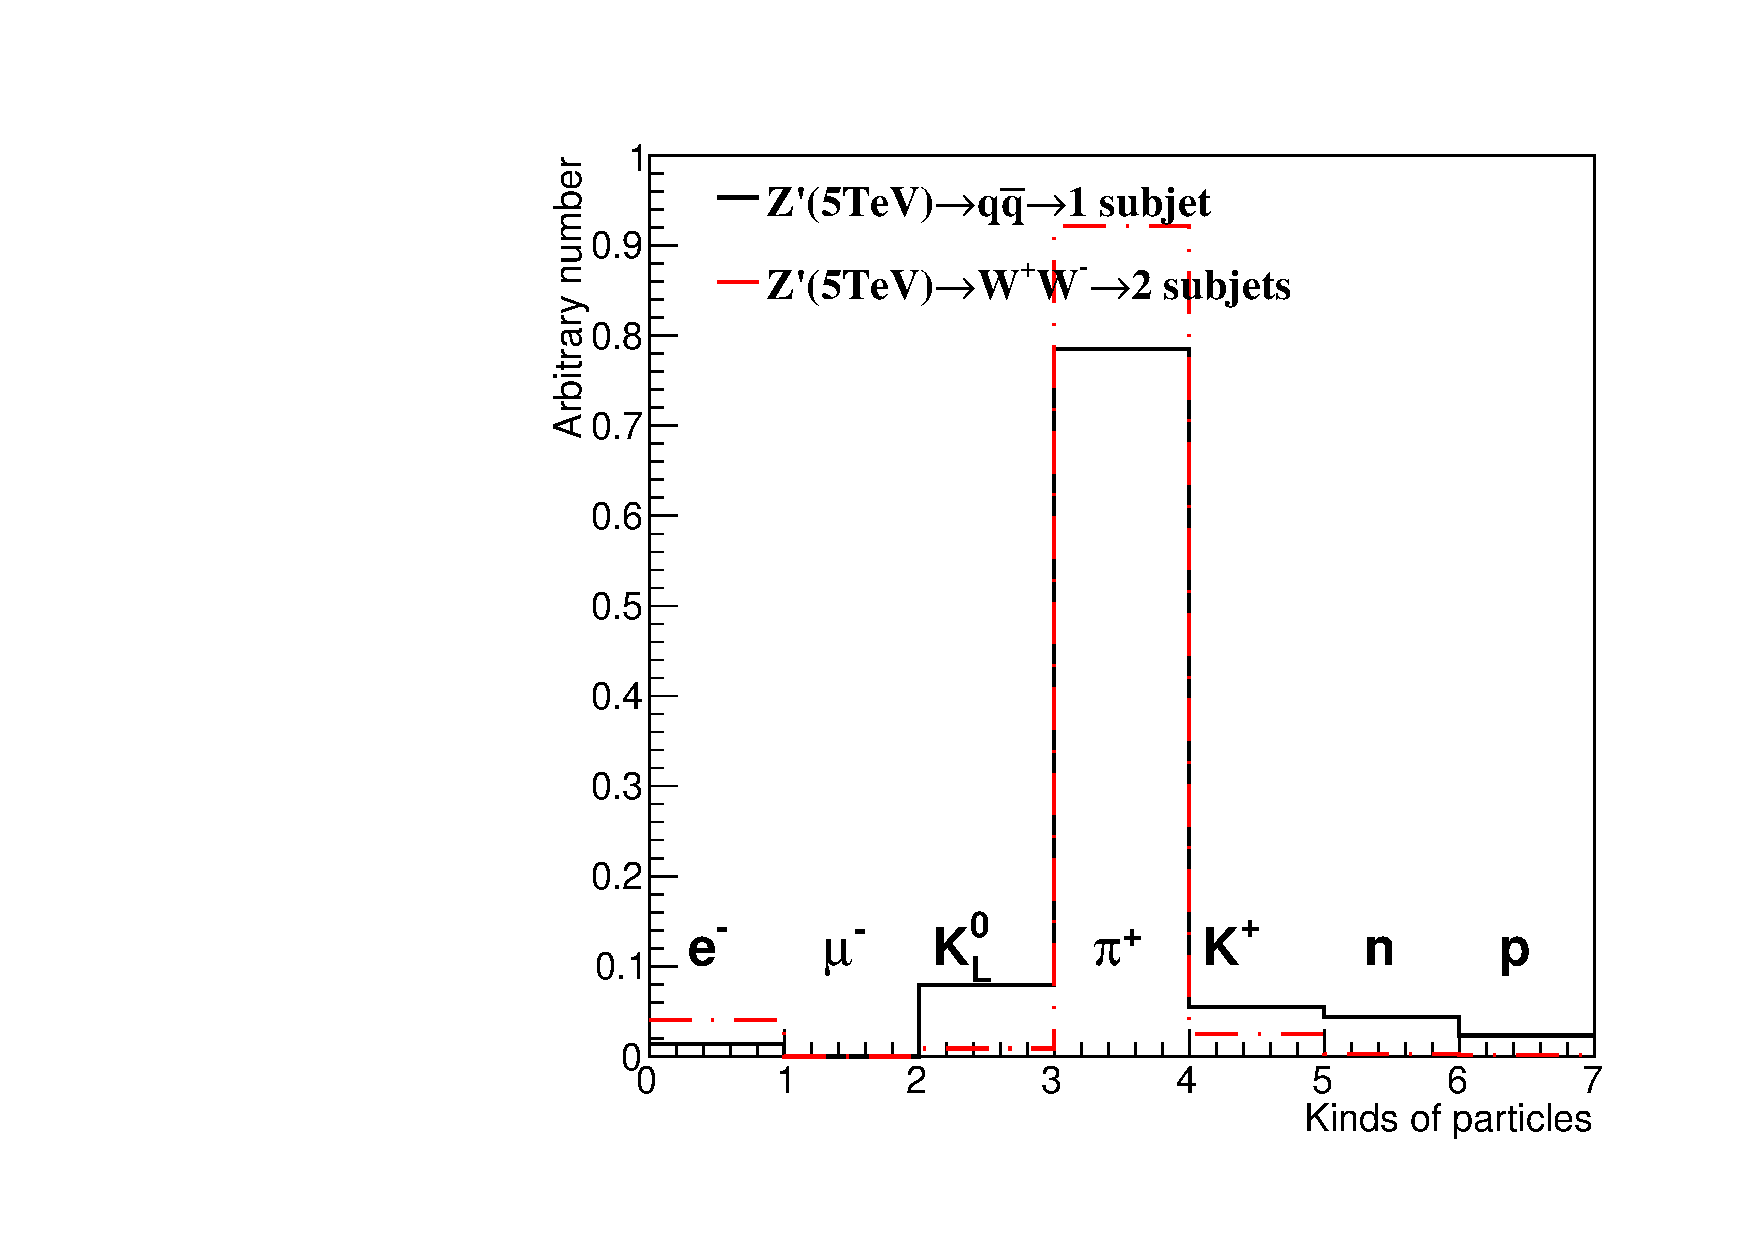
\includegraphics[width=0.45\textwidth]{/Users/ms08962476/singularity/TIming_Studies/Codes/5TeV/h_5TeV_Particles_Rank_PT_0.pdf}
   }
   \subfigure[Next-to-Trailing-T] {
   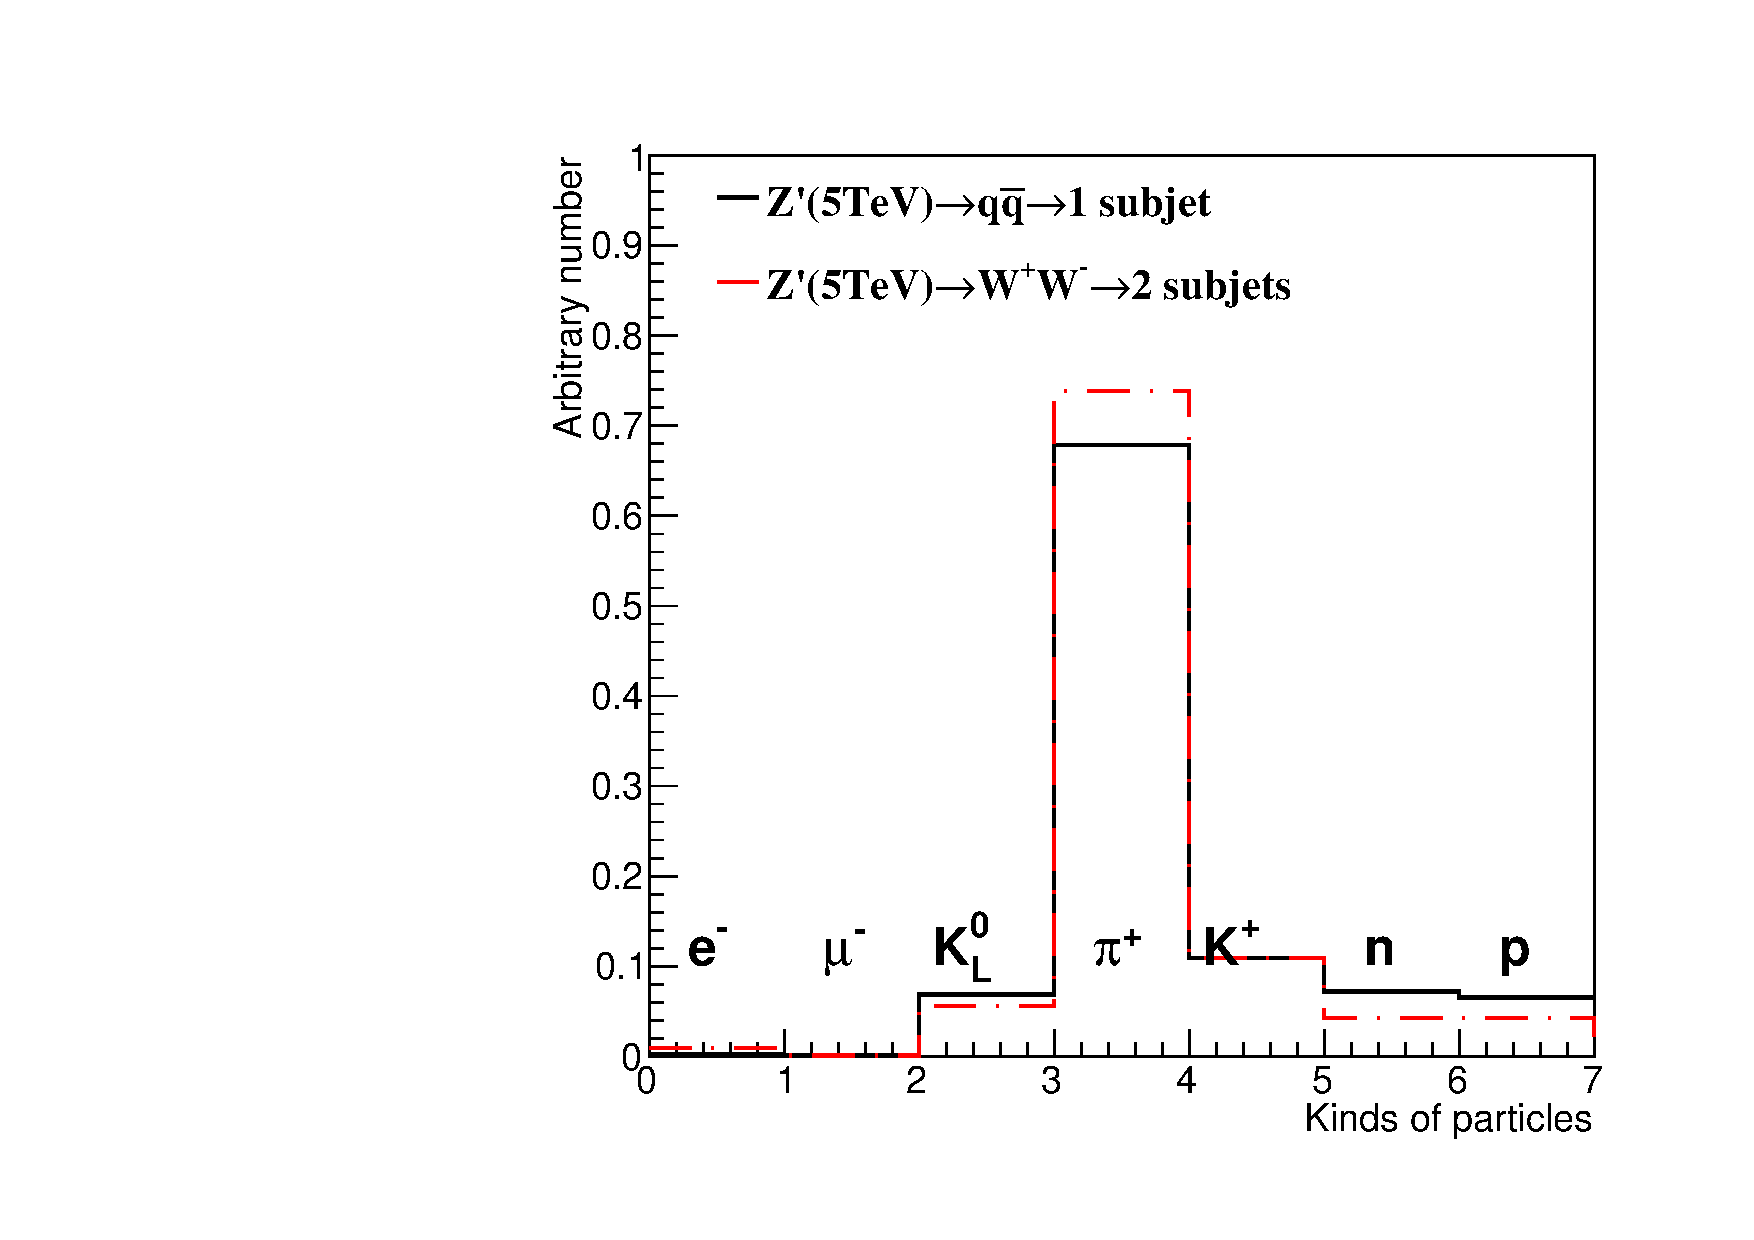
\includegraphics[width=0.45\textwidth]{/Users/ms08962476/singularity/TIming_Studies/Codes/5TeV/h_5TeV_Particles_Rank_T_1.pdf}
   }
    \subfigure[Next-to-Trailing-PT] {
   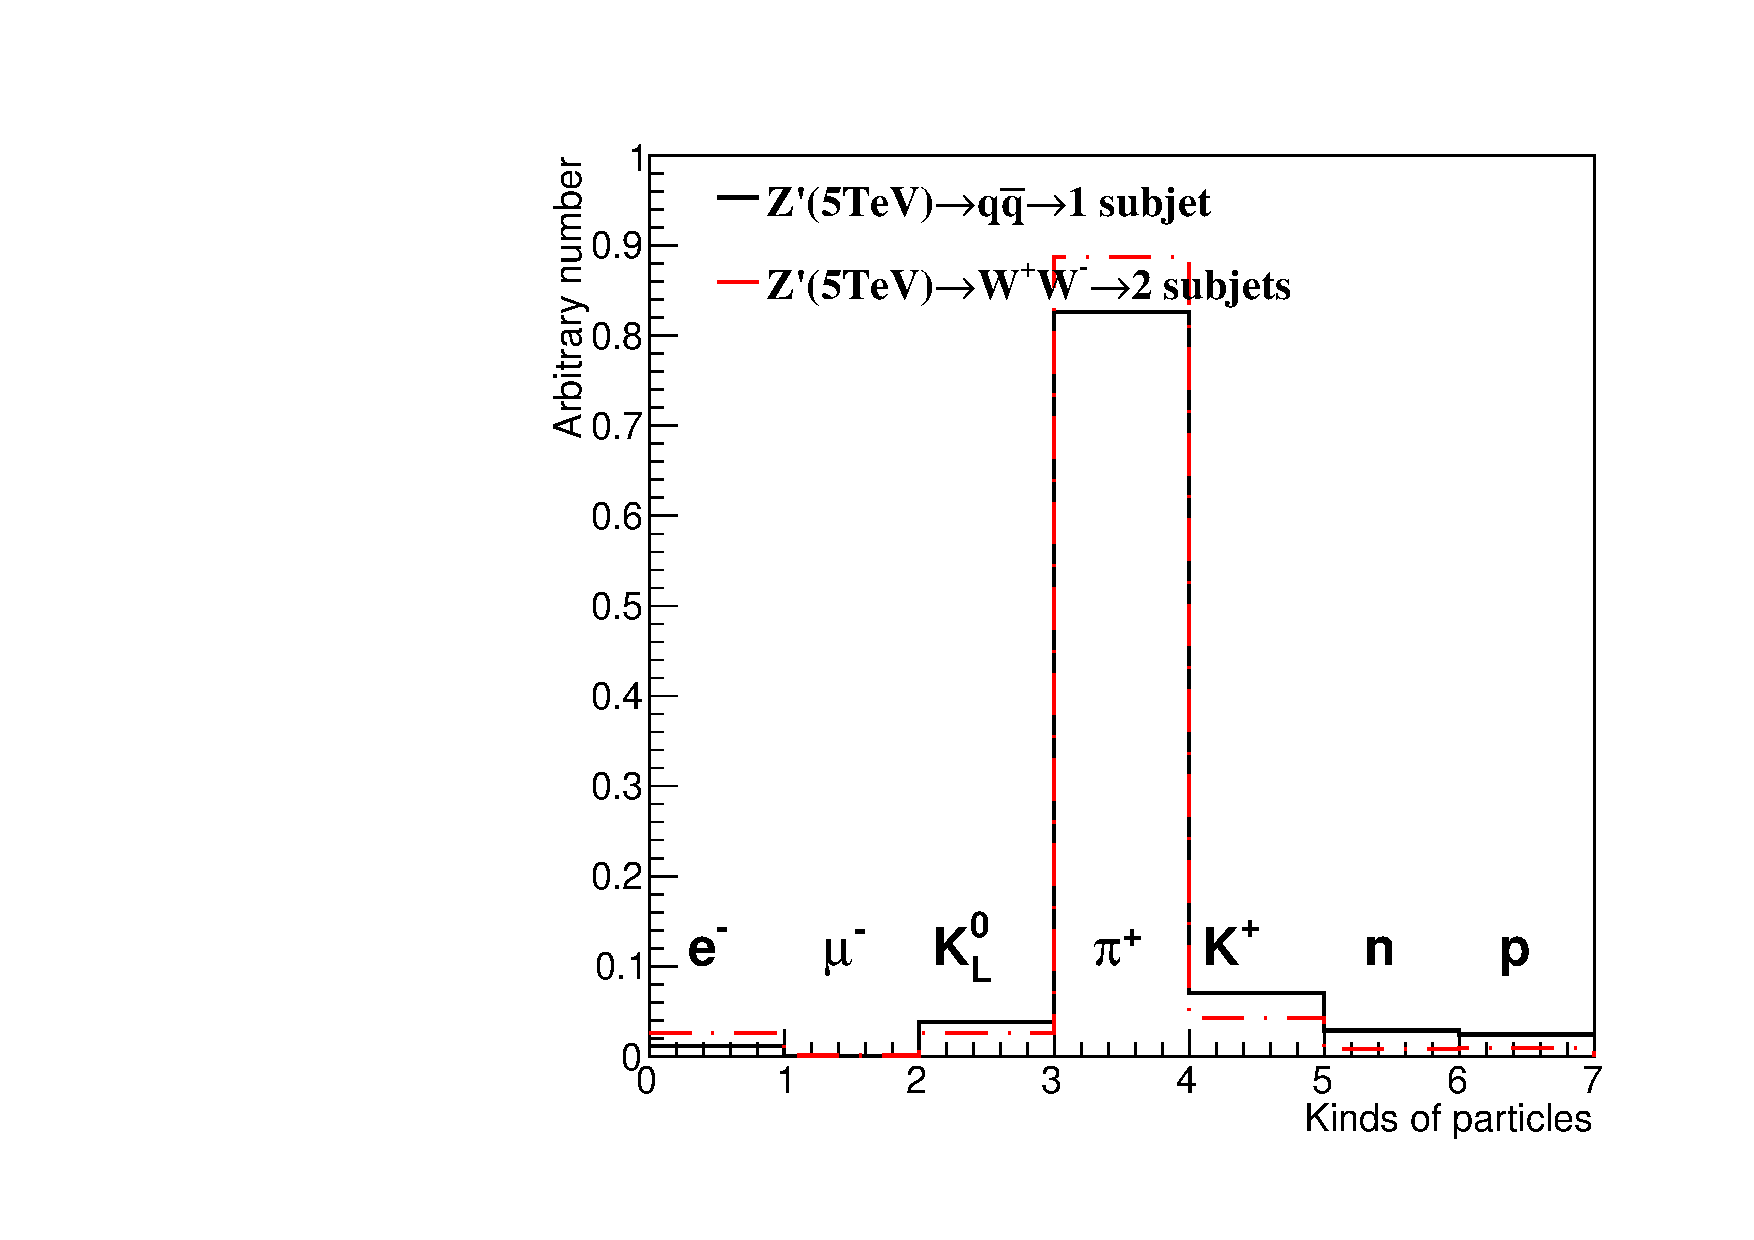
\includegraphics[width=0.45\textwidth]{/Users/ms08962476/singularity/TIming_Studies/Codes/5TeV/h_5TeV_Particles_Rank_PT_1.pdf}
   }
      \subfigure[Next-to-Next-to-Trailing-T] {
   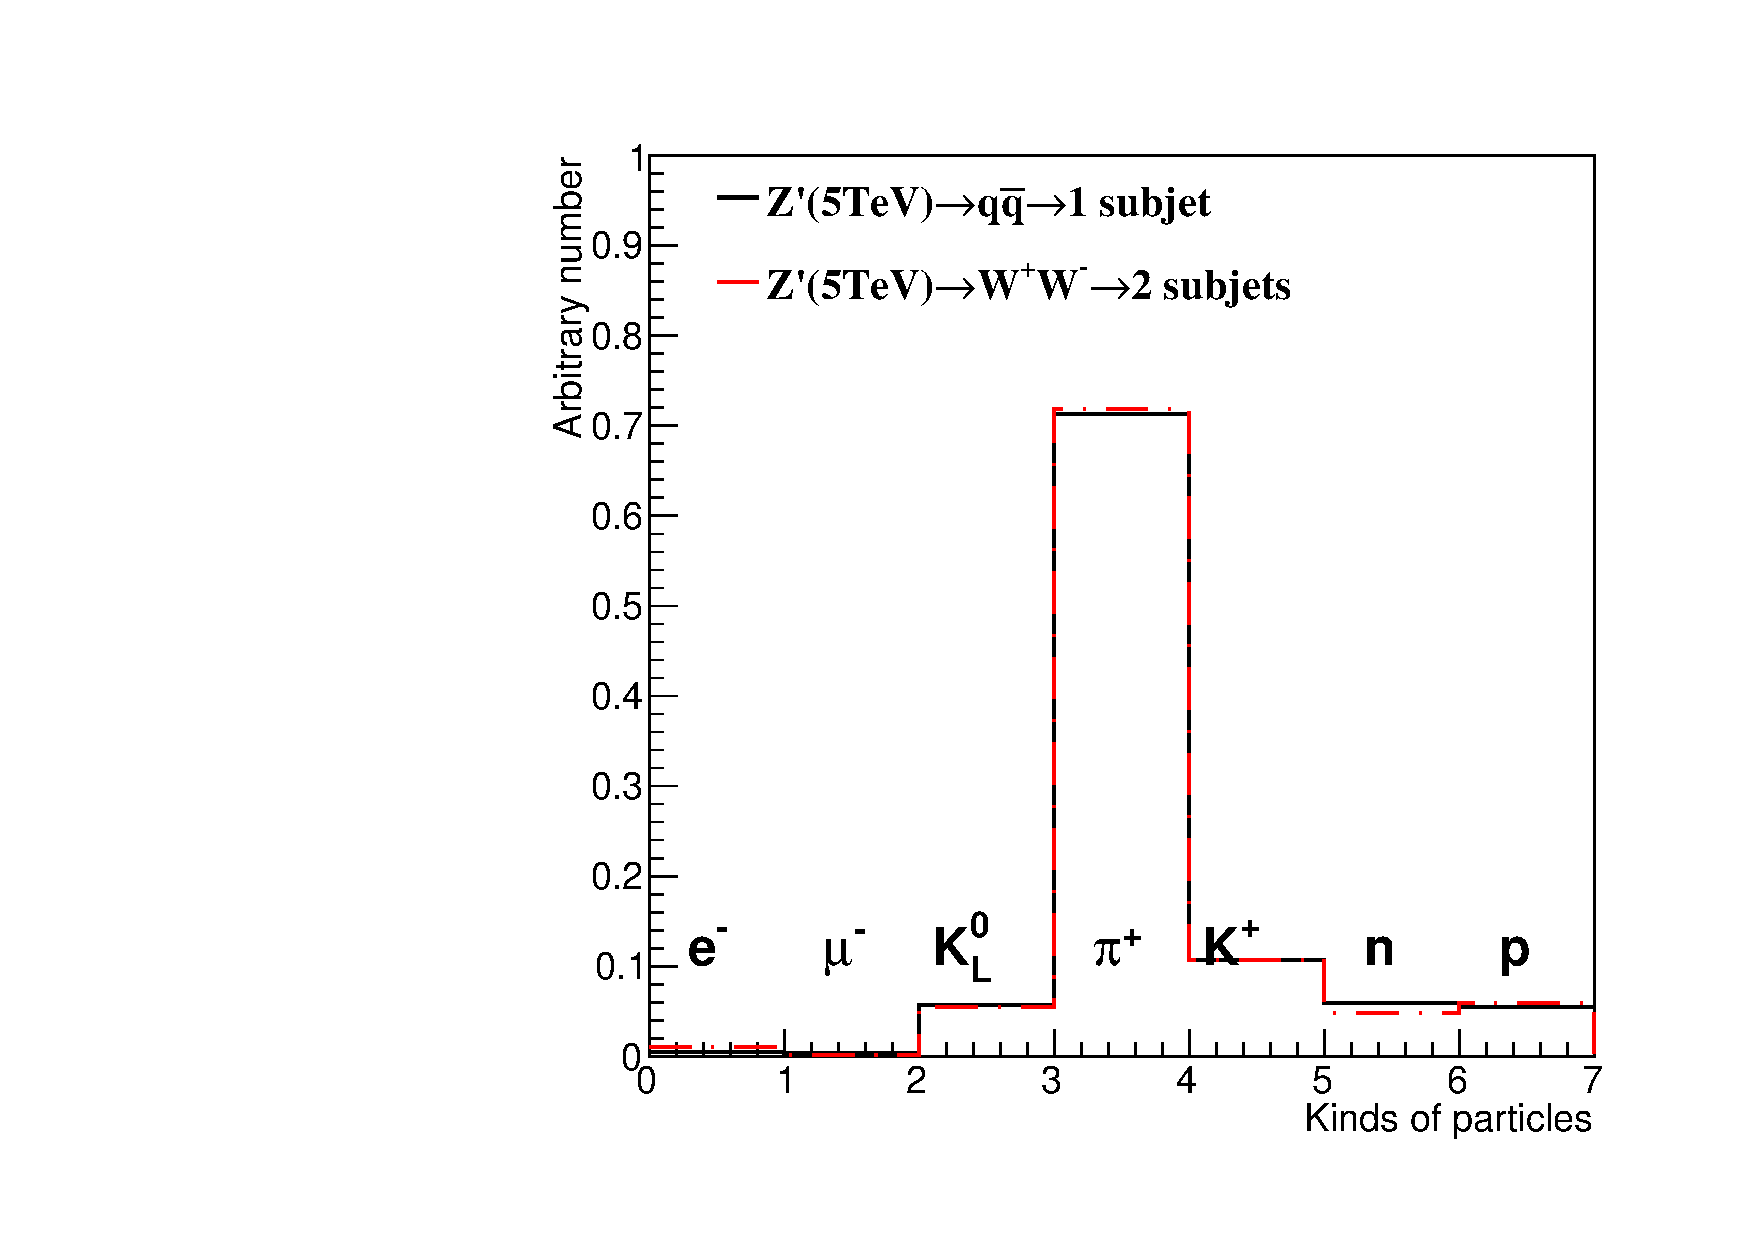
\includegraphics[width=0.45\textwidth]{/Users/ms08962476/singularity/TIming_Studies/Codes/5TeV/h_5TeV_Particles_Rank_T_2.pdf}
   }
    \subfigure[Next-to-Next-to-Trailing-PT] {
   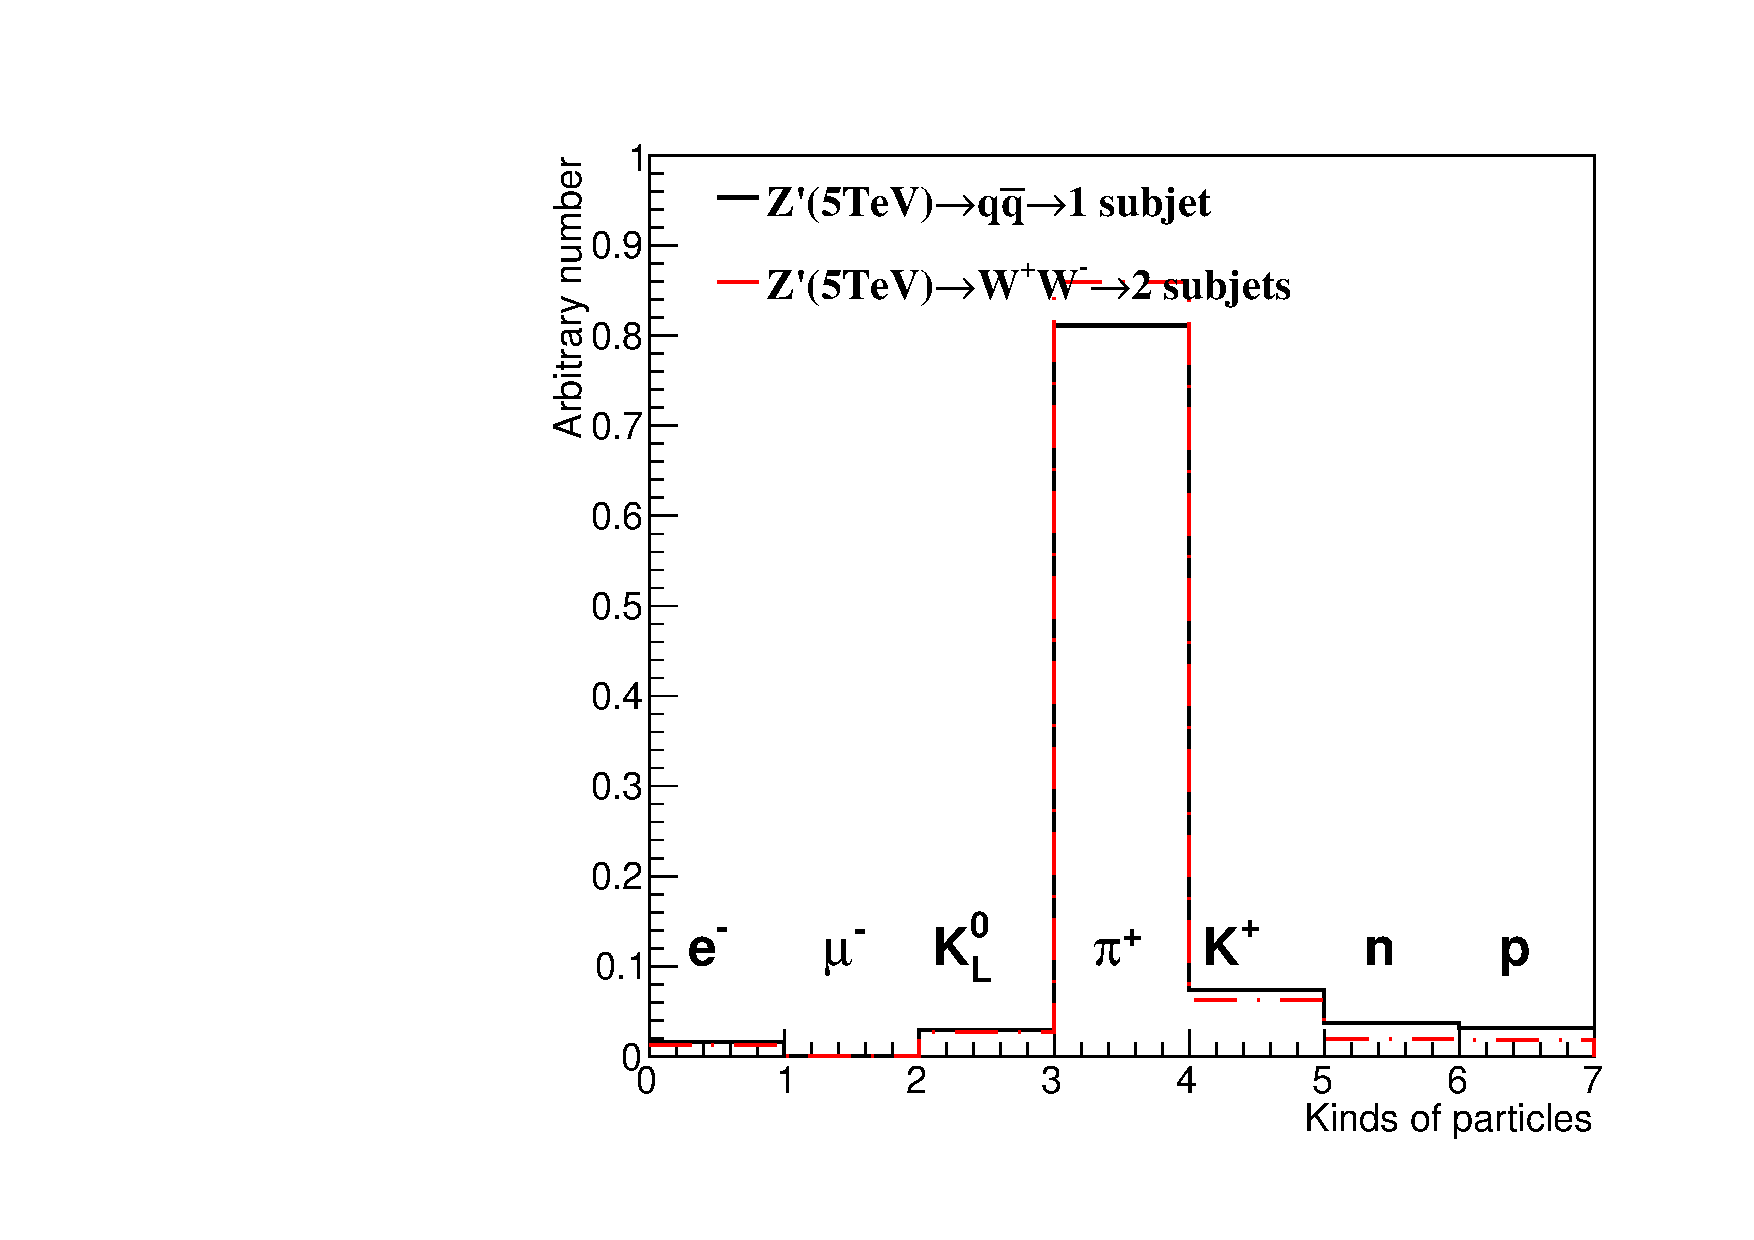
\includegraphics[width=0.45\textwidth]{/Users/ms08962476/singularity/TIming_Studies/Codes/5TeV/h_5TeV_Particles_Rank_PT_2.pdf}
   }

\end{center}
\caption{These are the particles ID of the different sorts of the trailing series with the definition of T and PT.}
\label{Particle_ID_1}
\end{figure}

\begin{figure}
\begin{center}
      \subfigure[Next-to-Next-to-Next-to-Trailing-T] {
   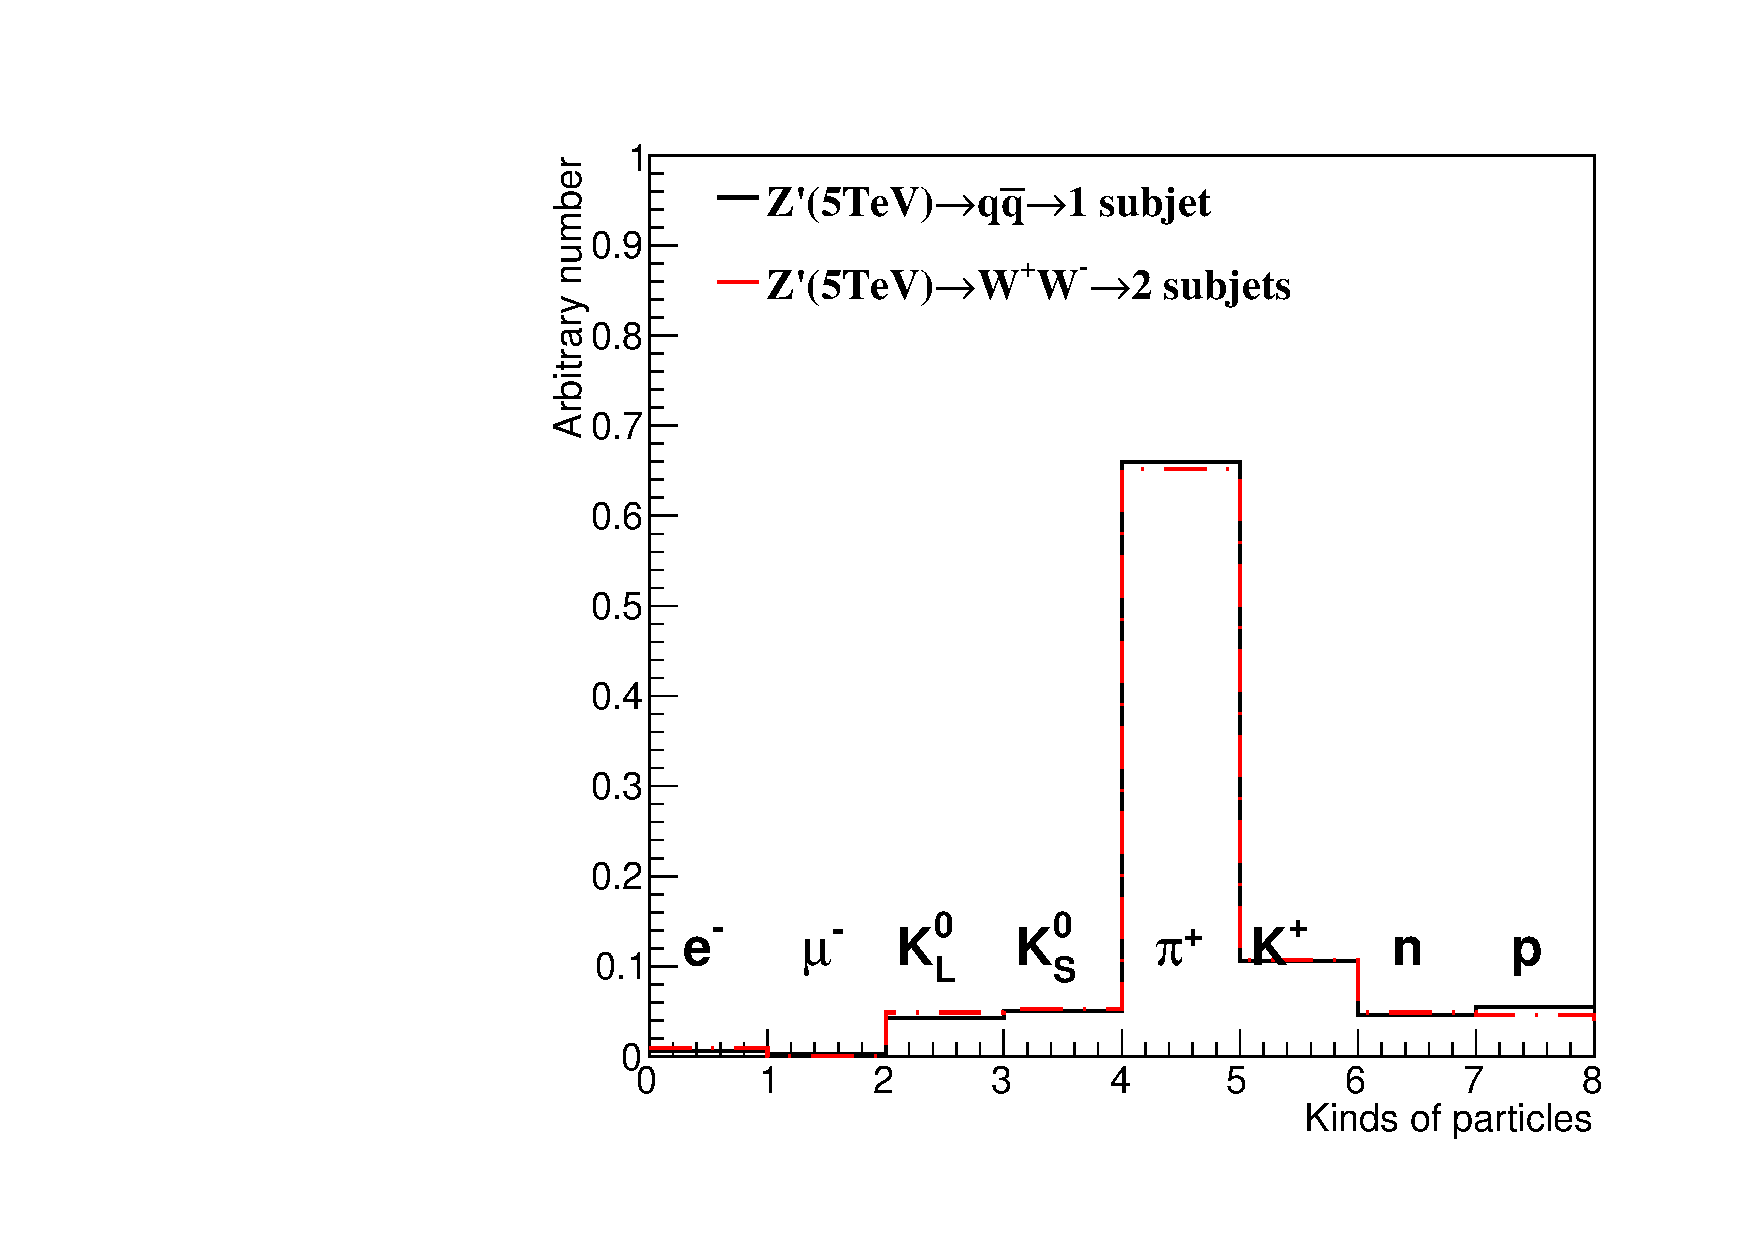
\includegraphics[width=0.45\textwidth]{/Users/ms08962476/singularity/TIming_Studies/Codes/5TeV/h_5TeV_Particles_Rank_T_3.pdf}
   }
    \subfigure[Next-to-Next-to-Next-to-Trailing-PT] {
   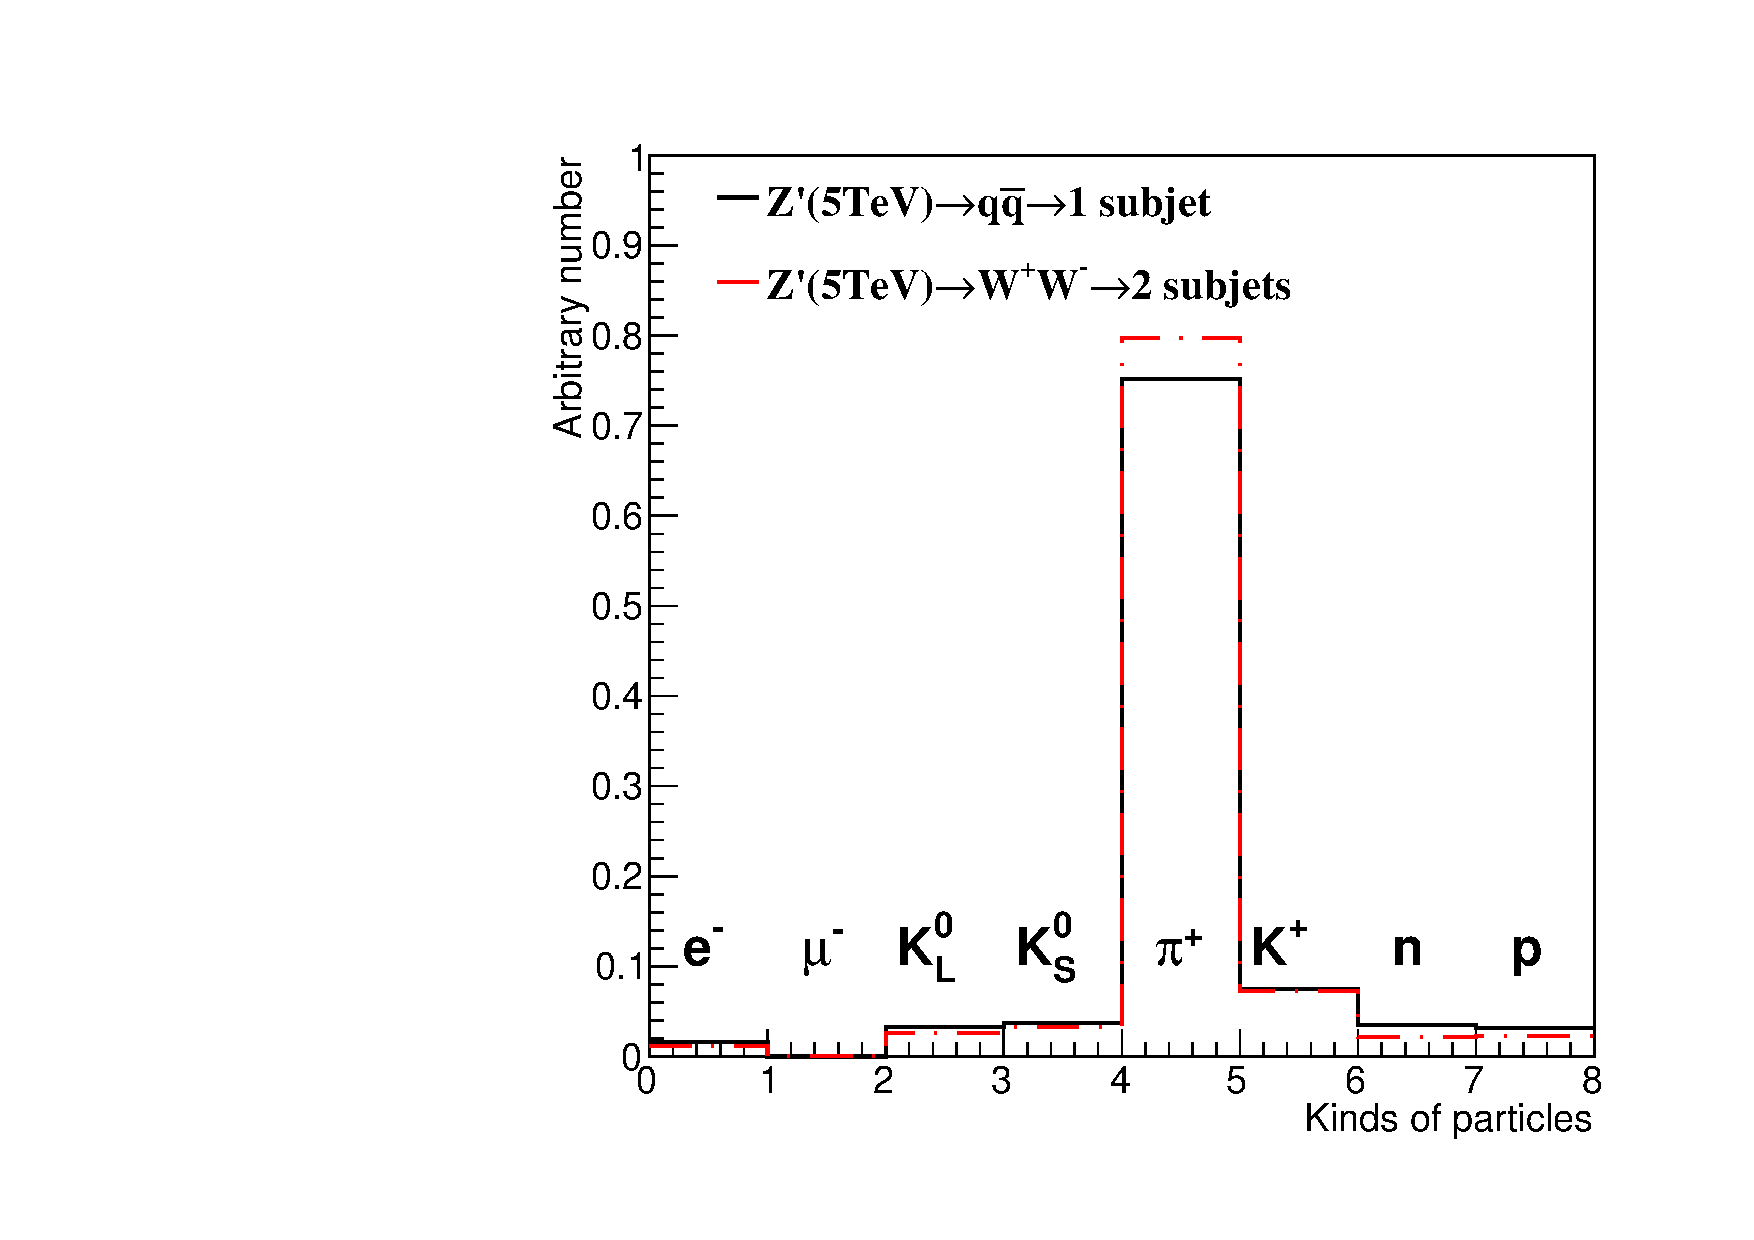
\includegraphics[width=0.45\textwidth]{/Users/ms08962476/singularity/TIming_Studies/Codes/5TeV/h_5TeV_Particles_Rank_PT_3.pdf}
   }
      \subfigure[Next-to-Next-to-Next-to-Next-to-Trailing-T] {
   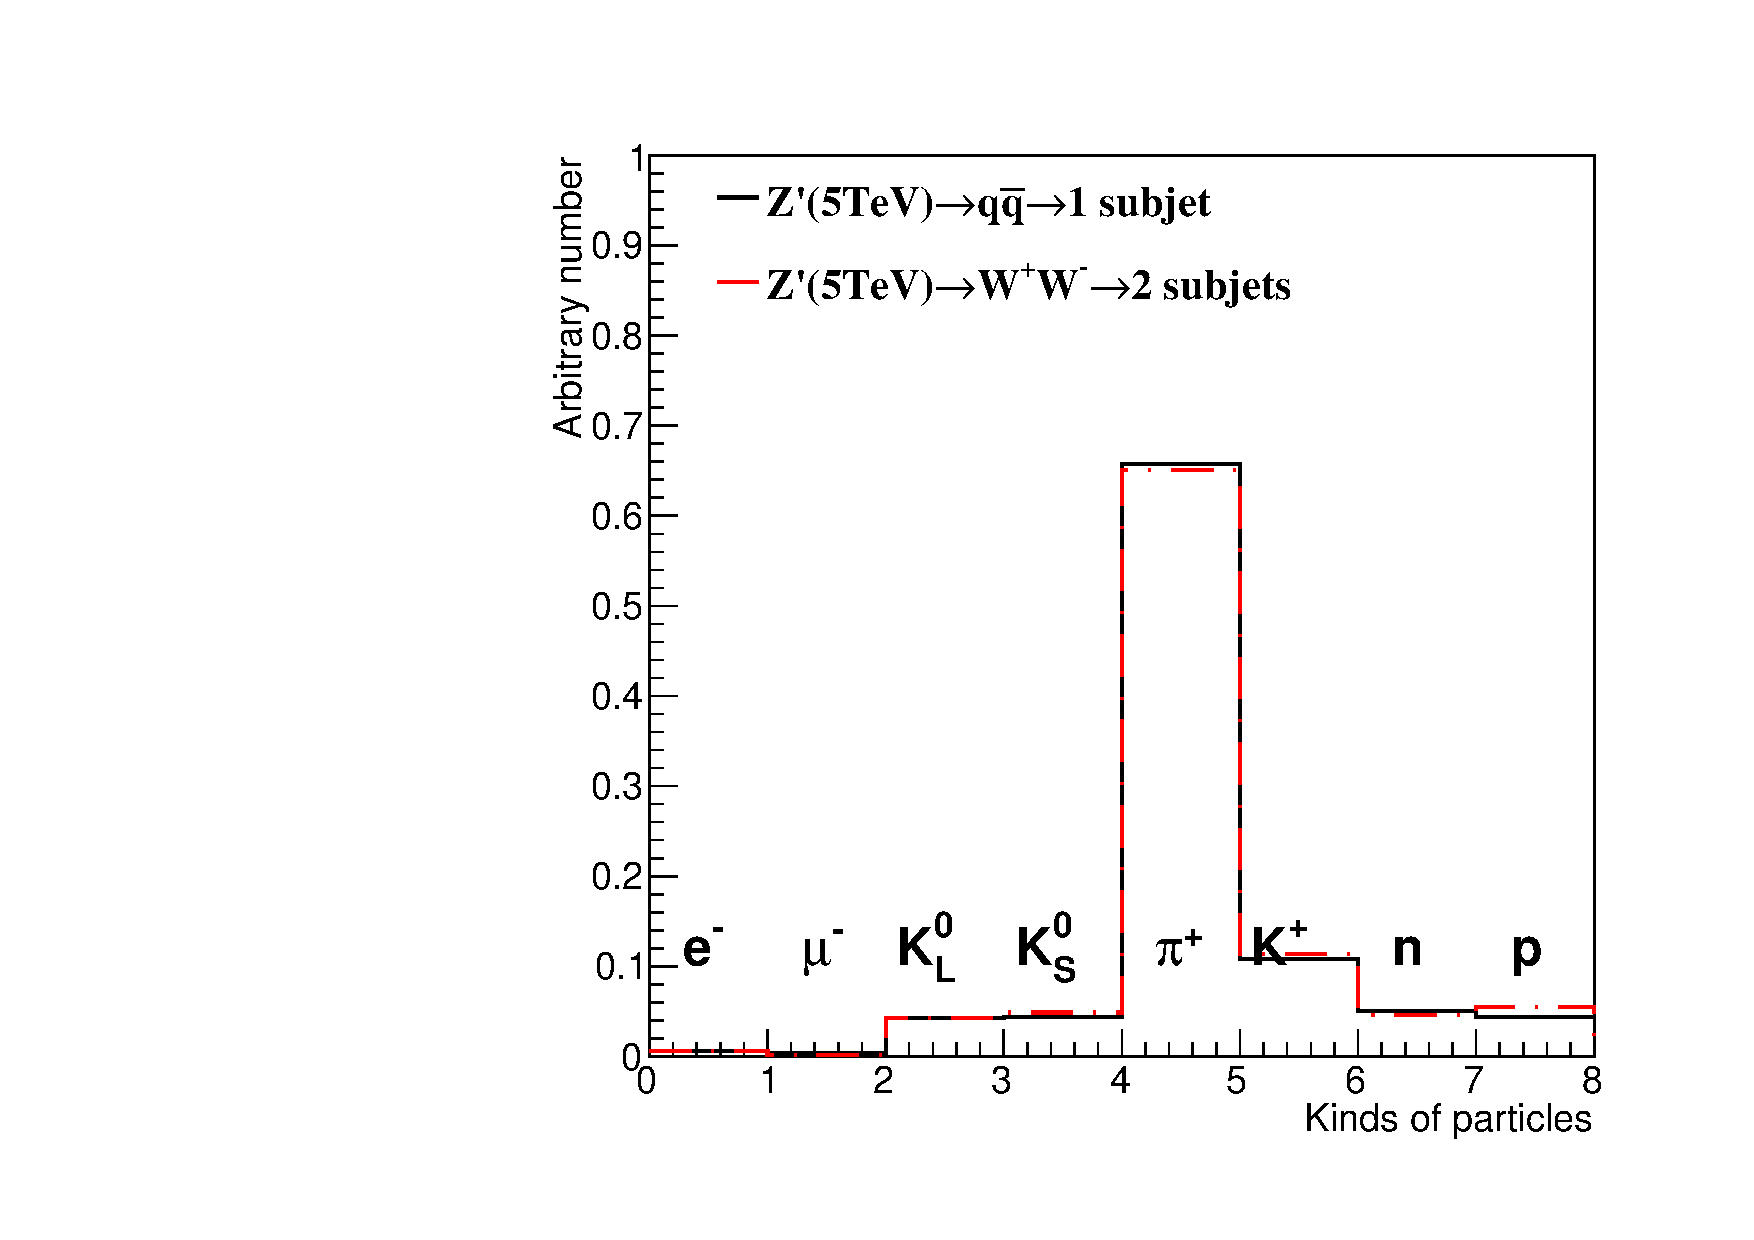
\includegraphics[width=0.45\textwidth]{/Users/ms08962476/singularity/TIming_Studies/Codes/5TeV/h_5TeV_Particles_Rank_T_4.pdf}
   }
    \subfigure[Next-to-Next-to-Next-to-Next-to-Trailing-PT] {
   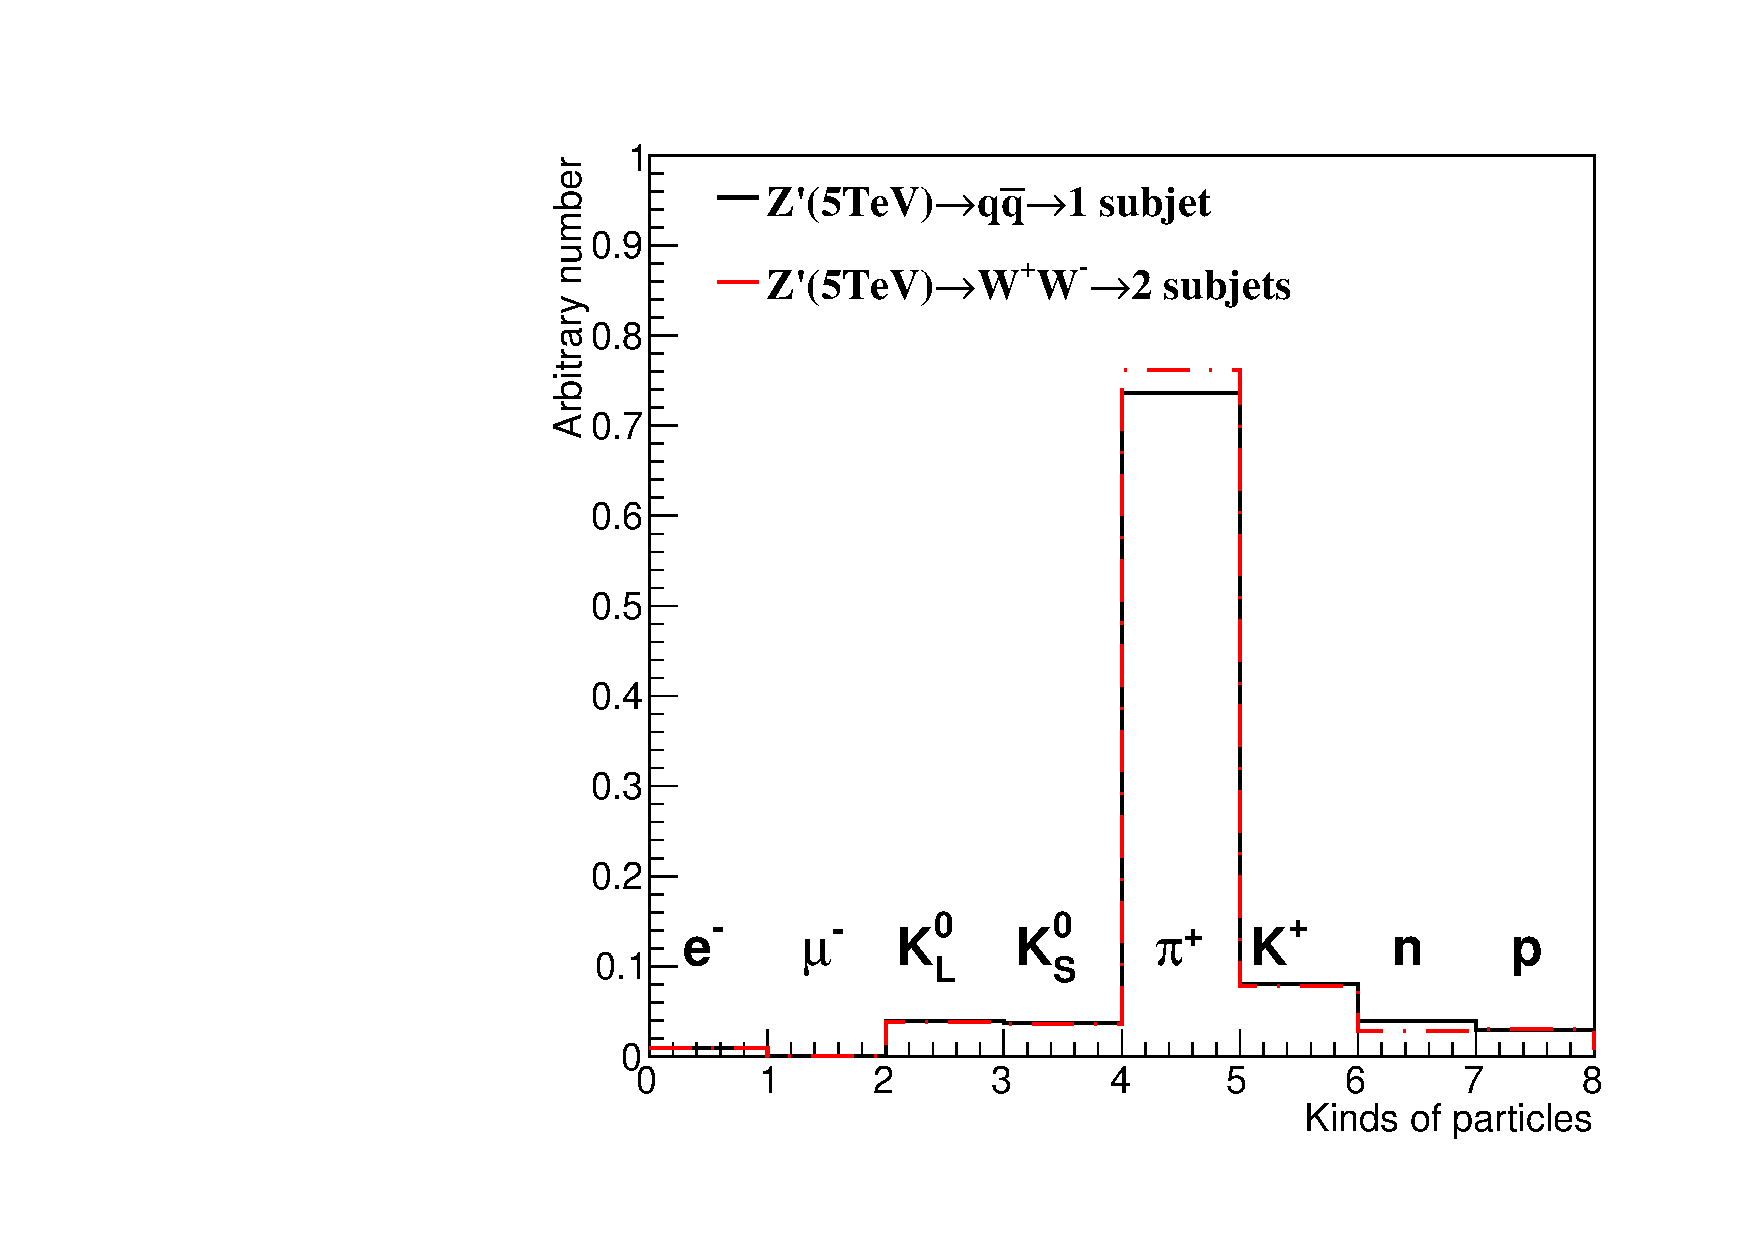
\includegraphics[width=0.45\textwidth]{/Users/ms08962476/singularity/TIming_Studies/Codes/5TeV/h_5TeV_Particles_Rank_PT_4.pdf}
   }

\end{center}
\caption{These are the particles ID of the different sorts of the trailing series with the definition of T and PT.}
\label{Particle_ID_2}
\end{figure}

%%%%%%%%%%%%%%% commented out 
\end{comment}
